\documentclass{beamer}
\usefonttheme{serif}
\usetheme{Boadilla}

\usepackage{graphicx}
\usepackage{listings}
\usepackage[T1]{fontenc}
\usepackage{lmodern}
\usepackage{xspace}
\usepackage{multicol}
\usepackage{textcomp}  % For currencies
\usepackage{tikz}
\usetikzlibrary{calc}

\title{\LaTeX{} and \TikZ}
\institute[]{Association for Computing Machinery \\ University of South Carolina}
\author{Hunter Damron}
\date{2019-01-30}

\lstset{basicstyle=\scriptsize\ttfamily,tabsize=2}
\newcommand{\samplecolumn}[2]{
	\begin{frame}
	\frametitle{#2}
	\begin{columns}[T]
		\begin{column}{0.5\textwidth}
			\lstinputlisting[language=TeX,breaklines=true]{#1}
		\end{column}
%		\pause
		\vrule
		\begin{column}{0.5\textwidth}
			\begin{minipage}{\linewidth}
				\input{#1}
			\end{minipage}
		\end{column}
	\end{columns}
	\end{frame}
}

\newcommand{\samplerow}[2]{
	\begin{frame}
	\frametitle{#2}
	\lstinputlisting[language=TeX,breaklines=true]{#1}
%	\pause
	\hrule
	\vspace*{4pt}
	\begin{minipage}{\linewidth}
		\input{#1}
	\end{minipage}
	\end{frame}
}

\let\oldLaTeX\LaTeX
\renewcommand{\LaTeX}{\oldLaTeX\xspace}
\newcommand{\TikZ}{Ti\textit{k}Z\xspace}
\newcommand{\XeTeX}{X\kern -.1667em\lower .5ex\hbox{\reflectbox{E}}\kern-.1em\TeX\xspace}
\newcommand{\ConTeXt}{Con\TeX{}t}
\newcommand{\LuaTeX}{Lua\TeX\xspace}

\begin{document}
	\renewcommand{\usepackage}[1]{}  % To allow using \usepackage in demos
	\maketitle

	\section{Overview}
	\begin{frame}
		\frametitle{Overview}
		\begin{itemize}
			\item What is \LaTeX and Why Should I Care?
			\item Basic Introduction to \LaTeX Code
			\item What is \TikZ and Why Shouldn't I Care Even Less?
			\item Basic Introduction to \TikZ Code
			\item Overview of Other Quite Nice \LaTeX Packages
			\item Outside uses of \LaTeX
		\end{itemize}
	\end{frame}

	\begin{frame}
		\frametitle{What and Why \LaTeX?}
		\begin{itemize}
			\item \LaTeX is a set of macros  written by Leslie Lamport on top of the typesetting system \TeX{} written by Donald Knuth~\cite{wiki}
			\item \LaTeX allows the author to focus on content rather than format
			\item Although the Microsoft Office Suite  has monopolized digital typesetting for personal use, \LaTeX survives in the academic world because of its superiority in typesetting mathematics.
		\end{itemize}
	\end{frame}

	\section{\LaTeX Quick Basics}

	\begin{frame}
		\frametitle{Sample \LaTeX Document}
		\begin{columns}[T]
			\begin{column}{0.5\textwidth}
			\lstinputlisting[language=TeX,breaklines=true]{Sample-Document.tex}
			\end{column}
			\begin{column}{0.5\textwidth}
			\begin{center}
				\framebox{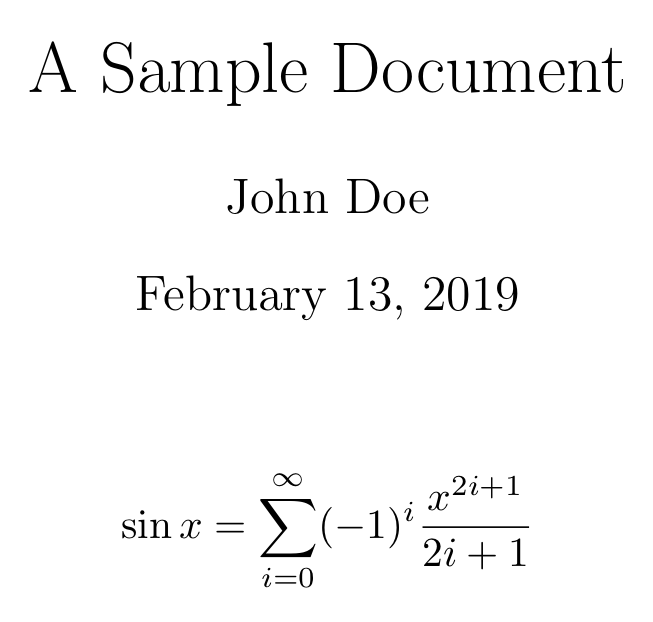
\includegraphics[width=0.95\linewidth]{Sample-Document}}
			\end{center}
			Cropped from a full page.
			\end{column}
		\end{columns}
	\end{frame}

	\samplerow{Math.tex}{Beautiful Math}
	\samplerow{Math-Symb.tex}{Catalog of Math Symbols}
	\samplerow{Math-Symb2.tex}{Catalog of Math Symbols}

	\begin{frame}[fragile]
		\frametitle{Catalog of Math Symbols}
		\begin{itemize}
			\item Most \LaTeX math commands are named appropriately as either their mathematical name (as in \verb$\forall$ $\forall$ and \verb$\exists$ $\exists$) or by their appearance (as in \verb$\cup$ $\cup$ and \verb$\cap$ $\cap$)
			\item To look up unknown commands, use Detexify~\cite{detexify}.
			\begin{center}
				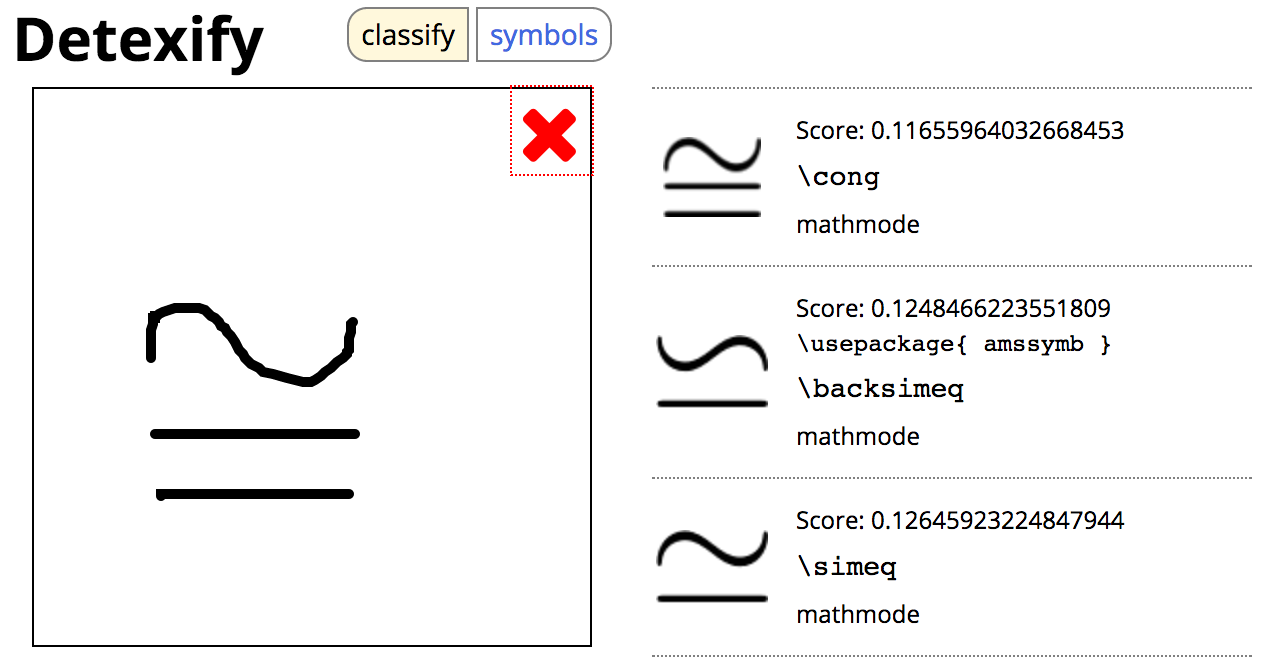
\includegraphics[width=0.7\linewidth]{Detexify}
			\end{center}
		\end{itemize}
	\end{frame}

	\samplerow{Image.tex}{Including Images}
	\samplerow{Lists.tex}{Organizing Lists}
	\samplerow{Table.tex}{Organizing Tables}

	\begin{frame}[fragile]
		\frametitle{Very Useful \LaTeX Packages}
		\begin{itemize}
			\item \verb$\usepackage{amsmath, amsthm, amssymb, mathtools}$~\cite{amsmath} provide many additional math capabilities
			\item \verb$\usepackage{graphicx}$ makes using graphics much more convenient
			\item \verb$\usepackage[T1]{fontenc}$ allows more characters to be typeset (loads font encoding \texttt{T1} which is more modern than default \texttt{OT1})
			\item \verb$\usepackage[utf8]{inputenc}$ allows Unicode characters in the document source
			\item \verb$\usepackage[...]{geometry}$ is used to modify page geometry
			\item \verb$\usepackage{array,tabularx}$ are useful extensions for building tables
			\item \verb$\usepackage{enumitem}$ extends the \texttt{itemize} and \texttt{enumerate} environments
			\item \verb$\documentclass{beamer}$ builds slide presentations (like this one)
		\end{itemize}
	\end{frame}

	\section{What is \TikZ}
	\begin{frame}
		\frametitle{What is \TikZ?}
		\begin{itemize}
			\item \TikZ is a \LaTeX package for typesetting simple graphics without an external image editor. Graphics are created from a textual description of the component shapes and their coordinates.
			\item \TikZ is built on another system called PGF which provides many useful extensions to \LaTeX, many unrelated to graphics.
		\end{itemize}
	\end{frame}

	\section{\TikZ Basics}

	\samplerow{Sample-Tikz.tex}{\TikZ Introduction}
	\samplecolumn{Tikz-Shorthand.tex}{\TikZ Commands and Shorthands}
	
	\begin{frame}[fragile]
		\frametitle{Common Commands in \TikZ}
		\begin{itemize}
			\item \verb$\path$ and \verb$\draw$ perform the same commands but \verb$\path$ does not draw anything (useful for intermediate steps in construction).
			\item \verb$\fill$ and \verb$\filldraw$ are shortcuts for \verb$\draw$ with solid color. 
			\item \verb$\node[options] at (coord) {Text};$
			\item \verb$\coordinate (name) at (location);$
			\item \verb$\draw (bottom left) rectangle (top right);$
			\item \verb$\draw (center) circle (radius);$
			\item \verb$\draw (center) ellipse (stretch: x and y);$
			\item B\'ezier curve \verb$\draw (start) .. controls (c1) and (c2) .. (end);$
			\item \verb$\draw (center) arc (start_ang:end_ang:radius);$ \\ (each \verb$ang$ in degrees)
		\end{itemize}
		Note each command can take \verb$[options]$ after the command statement.
	\end{frame}

	\begin{frame}[fragile]
		\frametitle{Common Options to Commands}
		\begin{itemize}
			\item \verb$ultra thin$, \verb$very thin$, \verb$thin$, \verb$thick$, \verb$very thick$, \verb$ultra thick$ control line thickness
			\item \verb$white$, \verb$black$, \verb$red$, \verb$green$, \verb$blue$, \verb$cyan$, \verb$magenta$, \verb$yellow$ are colors loaded by default; others can be created with the syntax \verb$(color)!(num)$ as in \verb$red!60$
			\item \verb$left$, \verb$right$, \verb$above$, \verb$below$ and any sensible combination tells nodes where to place text relative to their location
		\end{itemize}
	\end{frame}

	\samplerow{Tikz-Plot.tex}{Simple Plots in \TikZ}
	\samplerow{Positioning-Tikz.tex}{\texttt{positioning} library}

	\begin{frame}[fragile]
		\frametitle{Other Good \TikZ Libraries}
		\framesubtitle{Ref:\ \url{https://tex.stackexchange.com/a/42664}}
		\begin{center}
			\verb$\usetikzlibrary{...}$
		\end{center}
		\begin{multicols}{2}
		\begin{itemize}
			\scriptsize
			\item \texttt{arrows.meta} -- Arrow styles
			\item \texttt{automata} -- Finite automata
			\item \texttt{backgrounds} -- Background images
			\item \texttt{calc} -- Better calculations
			\item \texttt{calendar} -- Calendars
			\item \texttt{er} -- Entity-relationship diagrams
			\item \texttt{intersections} -- Shape intersections
			\item \texttt{mindmap} -- Mindmap diagrams
			\item \texttt{matrix} -- Organizing nodes
			\item \texttt{folding} -- Printing 3D shapes
			\item \texttt{patterns} -- Patterned shading
			\item \texttt{petri} -- Petri net diagrams
			\item \texttt{plothandlers} -- Better plots
			\item \texttt{plotmarks} -- Plot nodes
			\item \texttt{shapes.*} -- Many shapes
			\item \texttt{topaths} -- Better paths
			\item \texttt{trees} -- Trees and graphs
		\end{itemize}
		\end{multicols}
	\end{frame}

	\begin{frame}
		\frametitle{More Exotic \LaTeX}
		\fontsize{9}{\baselineskip}
		\begin{itemize}
			\item Extensions to \LaTeX which are more compatible with modern constructs like Unicode and provide better programming ability: \LuaTeX\footnote{\url{luatex.org}}, \XeTeX\footnote{\url{tug.org/xetex/}}, \ConTeXt\footnote{\url{wiki.contextgarden.net}}
			\item Literate Programming: Shortly after the creation of \TeX, Donald Knuth introduced the idea of weaving code into documentation as literate programming in his WEB\footnote{\url{www.ctan.org/pkg/web}} system. Although WEB was originally only for Pascal, modern alternatives include CWEB\footnote{\url{www.ctan.org/pkg/cweb}}, noweb\footnote{\url{https://www.cs.tufts.edu/~nr/noweb/}}, (all languages), Literate Haskell\footnote{\url{wiki.haskell.org/Literate_programming}}, knitr\footnote{\url{yihui.name/knitr/}} (R), Jupyter notebook\footnote{\url{jupyter.org}} (all languages; more than just \LaTeX)
			\item MathJax for \LaTeX math in the web\footnote{\url{www.mathjax.org}}
		\end{itemize}
	\end{frame}

	\begin{frame}[fragile]
		\frametitle{References}
		\begin{thebibliography}{9}
			\vspace*{-0.1em}
			\setbeamertemplate{bibliography item}[text]
			\bibitem{latexdoc} \LaTeX Documentation \url{www.latex-project.org/help/documentation/usrguide.pdf}
			\bibitem{amsmath} Documentation for \texttt{amsmath} package \url{www.latex-project.org/help/documentation/amsldoc.pdf}
			\bibitem{detexify} Detexify \url{http://detexify.kirelabs.org}
			\bibitem{minimaltikz} ``A very minimal introduction to \TikZ'' \url{https://cremeronline.com/LaTeX/minimaltikz.pdf}
			\bibitem{overleaftikz} Another Simple Introduction to \TikZ \url{www.overleaf.com/learn/latex/TikZ_package}
			\bibitem{tikzdoc} \TikZ and PGF Manual \url{http://ctan.math.illinois.edu/graphics/pgf/base/doc/pgfmanual.pdf}

			\bibitem{git}
			\href{https://github.com/latex3/latex2e.git}{\LaTeXe{} Open Source Repository}
			\bibitem{wiki}
			\href{https://en.wikipedia.org/wiki/LaTeX}{\LaTeX Wikipedia Page}
		\end{thebibliography}
	\end{frame}

	\begin{frame}
		\frametitle{My Projects}
		\begin{itemize}
			\item \texttt{shorthand}\footnote{\url{github.com/hdamron17/TeX-Notes.git}} package for taking notes
			\begin{itemize}
				\item This is especially useful if you are taking a physics lab
			\end{itemize}
			\item Noweb literate programming build system \texttt{noweb-make}\footnote{\url{github.com/hdamron17/noweb-make}} -- embeds source code beside output text and images
			\begin{itemize}
				\item Hacky but gets the job done for C/C++, Python, and Matlab
				\item Easily extensible for other languages
			\end{itemize}
			\item Package \texttt{eukleides}\footnote{\url{github.com/hdamron17/eukleides-tex.git}} (work in progress) for embedding geometric graphics created using the eukleides system in \LaTeX. Eukleides graphics specify connections between items but not the dimensions of the items themselves (i.e.\ you just want a generic triangle but do not care about its coordinates)
			\item This presentation\footnote{\url{github.com/hdamron17/tex-tikz-prez.git}} (to be put on GitHub shortly along with all \LaTeX sources)
		\end{itemize}
	\end{frame}
\end{document}